%%%%%%%%%%%%%%%%%%%%%%%%%%%%%%%%%%%%%%%%%%%%%%%%%%%%%%%%%%%%%%%%%%%%%%%%%%%%%%%%
% event_selection.tex: 
%%%%%%%%%%%%%%%%%%%%%%%%%%%%%%%%%%%%%%%%%%%%%%%%%%%%%%%%%%%%%%%%%%%%%%%%%%%%%%%%
\chapter{Event Selection}
\label{sec:event_selection_chapter}
%%%%%%%%%%%%%%%%%%%%%%%%%%%%%%%%%%%%%%%%%%%%%%%%%%%%%%%%%%%%%%%%%%%%%%%%%%%%%%%%

If a \WR boson and heavy neutrino \nul existed at a mass scale and coupling strength accessible 
at the LHC, evidence of them would manifest as an excess of events relative to expected backgrounds 
where two high-$p_{T}$ jets and two high-$p_{T}$, same flavor charged leptons were reconstructed.  
Charged leptons and jets were reconstructed and identified using the silicon tracker, the ECAL and 
HCAL, and the muon detectors.  In events where two same flavor charged leptons, and two jets were 
reconstructed, additional selections were applied to increase the sensitivity of this search to 
high-mass \WR and \nul signatures.

\section{Online Event Selection}
\label{sec:triggers}
Charged leptons that came from proton-proton interactions were identified by the trigger system.  Based 
on the multiplicity and energy of charged leptons, the trigger system selected events during 
collisions, and saved these events to permanent storage for further analysis.  The triggers presented 
here selected events in two steps.  In the first step, one or more Level-1 triggers were 
required to fire.  Then, in regions where Level-1 triggers fired, local reconstruction was run to 
build calorimeter and muon detector hits into granular, 3D energy clusters.  In the second step, 
a High Level trigger applied selection cuts to the 3D energy clusters.  If 
enough energy clusters (1 or 2, depending on the trigger) passed these selections, hits in the tracker 
layers were reconstructed into interaction vertices and charged particle tracks.  Track endpoints 
were then extrapolated along track trajectories to the calorimeters and muon detectors.  Extrapolated 
tracks that passed within $\Delta R < 0.1$ of an ECAL cluster were identified as electron (e) 
candidates, and extrapolated tracks that passed within the same distance of a muon detector cluster 
were identified as muon ($\mu$) candidates.  Final High Level trigger selections were applied to 
tracks in these e,$\mu$ candidates, and if the selections were passed the entire event was saved 
to permanent storage.  Specific selections used in different Level-1 and High Level triggers are 
discussed next.

Events used in the ee channel \WR search ($pp \rightarrow \WR \rightarrow eejj$) were first selected by Level-1 triggers 
that required: 

\begin{itemize}
	\item At least 40 GeV of energy was measured in one ECAL supercluster (SC), defined as a 5 $\times$ 5 crystal region.
	\item Or, at least 22 GeV of energy was measured in one SC, and at least 10 GeV of energy was measured in 
		another, non-overlapping SC.
\end{itemize}

Then, events were saved to permanent storage if the following double electron High Level trigger requirements 
were met: 

\begin{itemize}
	\item Two non-overlapping ECAL SCs were detected with energy $>$ 33 GeV.
	\item For each SC:
	\begin{itemize}
		\item The ratio of hadronic energy in the tower behind the SC to the SC energy was low, $\frac{E_{HCAL}}{E_{SC}} < 0.15$ in the barrel, $< 0.1$ in the endcap.
		\item For SCs in the barrel or endcap, 90\% of the SC energy was measured in an $(\eta, \phi)$ region that was two crystals wide in $\eta$.
		\item For SCs in the barrel, a reconstructed track with hits in at least two pixel tracker layers extrapolated to the $z_{SC}$ 
			SC center within 2.3 \cm, and the $(\eta_{SC}, \phi_{SC})$ SC center within the $(\eta, \phi)$ area of one ECAL crystal.
	\end{itemize}
\end{itemize}

The High Level trigger selections for electrons differ between the barrel and endcap regions because the ECAL 
crystal sizes and orientations relative to the $x$ and $y$ axes differ between the barrel and endcap, as 
explained in Chapter \ref{sec:experiment_chapter}.

A second set of ee channel events were used only to estimate backgrounds.  These events were first 
selected online using a Level-1 trigger that required $>$ 30 GeV of energy be measured in an ECAL SC 
with $|\eta| < 2.1$.  Following the Level-1 selection, events were saved to permanent storage if the 
following double electron High Level trigger requirements were met:

\begin{itemize}
	\item One SC was detected with energy $>$ 30 GeV.
	\item For the SC with energy $>$ 30 GeV:
	\begin{itemize}
		\item For SCs in the barrel or endcap, 90\% of the SC energy was measured in an $(\eta, \phi)$ region that was two crystals wide in $\eta$.
		\item The ratio of hadronic energy in the tower behind the SC to the SC energy was low, $\frac{E_{HCAL}}{E_{SC}} < 0.055$ in the barrel, $< 0.07$ in the endcap.
		\item In a cone of radius $\Delta R =$ 0.3 centered on the SC ($\thicksim$900 ECAL crystals, $\thicksim$35 HCAL towers in the cone):
		\begin{itemize}
			\item The fraction of the total ECAL energy in the cone not associated with the SC is low, $\frac{E_{ECAL}}{E_{SC}} < 0.225$ in the barrel, $< 0.121$ in the endcap.
			\item The total HCAL energy in the cone is small compared to the SC energy, $\frac{E_{HCAL}}{E_{SC}} < 0.155$ in the barrel, $< 0.16$ in the endcap.
		\end{itemize}
		\item For SCs in the barrel or endcap, a reconstructed track with hits in at least two pixel tracker layers extrapolates to the 
			$z_{SC}$ SC center within 1 \cm, and the $(\eta_{SC}, \phi_{SC})$ SC center within the $(\eta, \phi)$ area of $\frac{1}{2}$ ECAL crystal.
		\item For SCs in the barrel or endcap, the SC energy and the matching reconstructed track momentum cannot differ by more than 50\%
	\end{itemize}
	\item A second SC was detected with energy $>$ 4 GeV.
\end{itemize}


Events used in the muon channel \WR search ($pp \rightarrow \WR \rightarrow \mu\mu jj$) were first selected online using 
a Level-1 trigger that required $>$ 16 GeV of momentum be measured in a muon DT or CSC detector.  Following 
the Level-1 selection, events were saved to permanent storage if the following single muon High Level trigger 
requirements were met: 

\begin{itemize}
	\item The same requirements were applied to muon candidates in the barrel and endcap.
	\item A global curve representing a muon candidate was fit to a reconstructed track and at least one muon detector hit with $\chi^{2}/nDOF <$ 20.
	\item In the $(x,y)$ plane, the distance between the origin of the muon track and the primary vertex was $<$ 1 \mm.
	\item The reconstructed muon track had $p_{T} >$ 50 GeV.
\end{itemize}

A second set of $\mu\mu$ channel events were used only to estimate backgrounds.  These events were first 
selected online by a Level-1 trigger, which required $>$ 20 GeV of momentum be measured in a muon 
DT or CSC detector.  Following the Level-1 selection, events were saved to permanent storage if the 
following single muon High Level trigger requirements were met:

\begin{itemize}
	\item Unless noted otherwise, the same requirements were applied to muon candidates in the barrel and endcap.
	\item A global curve representing a muon candidate was fit to a reconstructed track and at least one muon detector hit with $\chi^{2}/nDOF <$ 20.
	\item In the $(x,y)$ plane, the distance between the origin of the muon track and the primary vertex was $<$ 1 \mm.
	\item The reconstructed muon track had $p_{T} >$ 22 GeV.
	\item In a cone of radius $\Delta R =$ 0.3 centered on the muon detector energy cluster ($\thicksim$900 ECAL crystals, $\thicksim$35 HCAL towers in the cone):
	\begin{itemize}
		\item The total ECAL energy in the cone is small compared to the muon cluster energy, $\frac{E_{ECAL}}{E_{\mu}} < 0.11$ in the barrel, $< 0.08$ in the endcap.
		\item The total HCAL energy in the cone is small compared to the muon cluster energy, $\frac{E_{HCAL}}{E_{\mu}} < 0.21$ in the barrel, $< 0.22$ in the endcap.
		\item The sum $p_{T,other}$ of all tracks in the cone excluding the muon track is small compared to the muon track $p_{T,\mu}$, 
			$\frac{p_{T,other}}{p_{T,\mu}} < 0.09$ in the barrel and endcap.
	\end{itemize}
\end{itemize}


As stated in Chapter \ref{wrBosonAndHeavyNu}, it is assumed that the $\WR$ decay cannot violate lepton 
flavor conservation.  As a result, the search presented here did not seek evidence of the LRS model in 
events with one electron, one muon and two jets in the final state.  However, events in the $e\mu$ channel 
($e\mu jj$ final state) were used to estimate backgrounds using a procedure described later.  The $e\mu$ 
channel events were first selected by a Level-1 trigger that required $>$ 16 GeV of momentum be 
measured in one muon DT or CSC detector.  Events that passed the Level-1 trigger were saved to permanent 
storage if the following electron $+$ muon High Level trigger requirements were met:

\begin{itemize}
	\item A global curve representing a muon candidate was fit to a reconstructed track and at least one muon detector hit with $\chi^{2}/nDOF <$ 20.
	\item In the $(x,y)$ plane, the distance between the origin of the reconstructed muon track and the primary vertex was $<$ 1 \mm.
	\item The reconstructed muon track had $p_{T} >$ 30 GeV.
	\item One ECAL SC was detected with energy $>$ 30 GeV.
	\item For the SC:
	\begin{itemize}
		\item The ratio of hadronic energy in the tower behind the SC to the SC energy must be low, $\frac{E_{HCAL}}{E_{SC}} < 0.15$ in the barrel, $< 0.1$ in the endcap.
		\item For SCs in the barrel or endcap, 90\% of the SC energy must be measured in an $(\eta, \phi)$ region that is two crystals wide in $\eta$.
		\item For SCs in the barrel, a reconstructed track with hits in at least two pixel tracker layers extrapolated to the 
			$z_{SC}$ SC center within 2.3 \cm, and the $(\eta_{SC}, \phi_{SC})$ SC center within the $(\eta, \phi)$ area of one ECAL crystal.
	\end{itemize}
\end{itemize}


\subsection{Data}
\label{sec:collisionData}

The LHC started colliding protons at $\sqrt{s} = 13\TeV$ center-of-mass energy in April 2015.  From 
April until mid August, proton bunches in each beam were separated by 50 \ns.  The data collected 
in this period, $\thicksim$0.2 fb$^{-1}$, was used to calibrate and align all CMS subdetector systems, but 
was not used in the search presented here for the following reason.  Before 2015 collisions began it 
was known that the amount of 50 \ns data collected would be small compared to the data collected with 
25 \ns bunch spacing.  As a result, the vast resources needed for physics analyses, like Monte Carlo simulations 
of SM processes used to estimate backgrounds, were only produced for data collected with 25 \ns bunch 
spacing.  The person-power needed to develop the same resources for 50 \ns data would have been 
detrimental to the quality of results produced with 25 \ns data.

The LHC stopped collisions in the second half of August and early September, evidenced by the plateau 
in Figure \ref{fig:lhc2015IntegLumi} \cite{lumi} during this time, to reconfigure the CERN accelerator system to 
deliver proton-proton (pp) collisions with 25 \ns between proton bunches.  The bunch spacing was decreased to 
increase the rate of pp collisions without increasing the number of interactions per pp collision event, 
which makes particle reconstruction and identification more difficult.  Collisions at $\sqrt{s} = 13\TeV$ 
resumed in September and continued until November 2015. During this period the LHC delivered approximately 
4.0 fb$^{-1}$ of data, but problems with the CMS magnet limited the amount of data recorded 
by CMS with the full 3.8 $\unit{T}$ magnetic field strength to 2.6 fb$^{-1}$.  The full 2.6 fb$^{-1}$ was used in this analysis, and was 
divided into two run periods - Run2015C and Run2015D.  All data from September until mid October 
was collected with similar beam conditions, like average instantaneous luminosity and the number of bunches 
per beam, and constituted run era Run2015C.  In mid October collisions stopped for $\thicksim$1.5 weeks for 
LHC maintenance, and to upgrade the LHC to deliver collisions with higher instantaneous luminosities, 
approaching $6 \times 10^{33} \frac{protons}{cm^{2}s}$.  Data collected after this upgrade and until the end 
of pp collisions in November constituted run era Run2015D.  As in Run2015C, all data in Run2015D was collected 
with similar beam conditions.  Comparing the two run eras in Table \ref{tab:collisionDatasets}, most of the 
data used in this analysis was collected in Run2015D.

\begin{figure}[h]
	\centering
	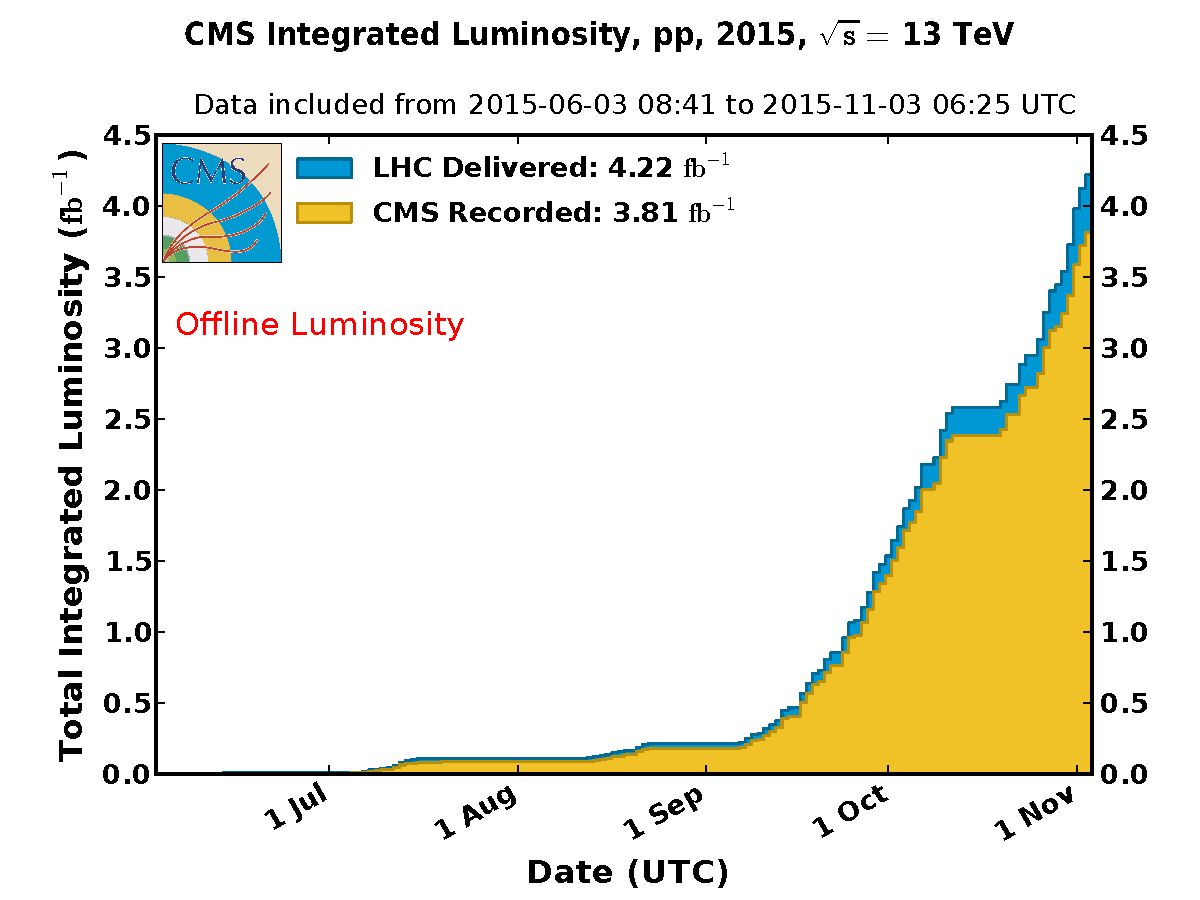
\includegraphics[width=1.0\textwidth]{figures/int_lumi_per_day_cumulative_pp_2015.pdf}
	\caption{Integrated luminosity delivered by the LHC and recorded by CMS in 2015.  Only data collected after 
	September 1st, corresponding to 25 \ns bunch spacing, was used in this search.}
	\label{fig:lhc2015IntegLumi}
\end{figure}

\begin{table}[h]
\caption{The amount of data collected in each run era.}
\label{tab:collisionDatasets}
\centering
\begin{tabular}{c|c}
Run Era & Int. Lumi (fb$^{-1}$) \\  \hline
	2015C &  0.02  \\
	2015D &  2.62  \\ \hline
\end{tabular}
\end{table}

After collision events were selected by High Level triggers, raw detector information was reconstructed into charged 
leptons, photons, and jets using procedures described later.  After the reconstruction process, the full 25 \ns 
2015 dataset collected by CMS was enormous ($\gtrsim 10^{4}$ terabytes), and contained much 
more information than what was needed by any individual physics analysis.  To expedite the transformation of 
collision data into a public physics result, reconstructed collision events from each run era were split into smaller 
datasets distinguished by the High Level triggers that selected the events.  As discussed earlier in 
Section \ref{sec:triggers}, collision events used in this analysis were selected if they had energy deposits consistent 
with at least one muon, at least two electrons, or at least one muon and one electron.  Events selected by the single 
muon triggers were assigned to the "SingleMuon" dataset, while those selected by the double electron and electron $+$ 
muon triggers were assigned to the "DoubleEG" (EG for electron gamma) and "MuonEG" datasets, respectively.  
The storage space consumed by these datasets largely came from object collections, representing quantities 
like individual hits in all tracker or calorimeter cells, that were not needed by the majority of physics 
analyses, including the one presented here.  Slimmed datasets were made by removing these object collections, and moving 
their important information into more general object collections, like the sole collection representing all 
reconstructed electrons.  Slimmed versions of the three datasets mentioned earlier were used in this 
analysis, and in each run era individual datasets were $\thicksim$5 terabytes or smaller.


%In addition to the trigger requirements discussed above, collision datasets are cleaned of events
%in which global reconstruction problems occurred within the detector.  These include events
%where no primary vertex is reconstructed, and when anomalous noise appears in the
%tracker, calorimeters, or muon detectors.  Furthermore, events identified as coming from
%interactions between a single proton beam and beam pipe gas or other foreign material are
%removed.


\section{Monte Carlo}
\label{sec:MC}

Monte Carlo (\MC) simulations were used in this search to model two types of processes.  The first 
type was Standard Model (SM) processes that resulted in the reconstruction of two charged leptons 
and two jets.  These included processes that produced two real charged leptons and two jets, like 
$pp \rightarrow Z+jets \rightarrow ll+jets$, and processes that produced multiple jets that 
were incorrectly reconstructed as charged leptons, like $pp \rightarrow W+jets \rightarrow l\nu+jets$.  
The second type was the \WR signal process $pp \rightarrow \WR \rightarrow l\nul \rightarrow lljj$ 
with different \mWR and \mnul masses.  
\MC simulations of both types of processes were produced by the CMS \MC production group 
in the following five step procedure.  In the first step, a \MC generator, like \PYTHIA or \MADGRAPH, simulated 
collision events between two protons in a vacuum, without any magnetic field or CMS detector 
components.  In simulations, the generator accounted for:

\begin{itemize}
	\item The energy carried by each proton into the collision (6.5 \TeV).
	\item How the incoming proton energy was distributed amongst constituent quarks and gluons according 
		to parton distribution functions (PDFs).
	\item The masses of the \WR, \nul and all particles in the SM.
	\item The coupling strengths between fermions and the bosons that mediated interactions.
\end{itemize}

Any unstable particles produced in the interaction, like a $Z$ or \WR boson, decayed according to 
their branching fractions to other particles, and any free quarks or gluons that were produced were 
run through a hadronization simulation that emulates jet production described in Chapter \ref{wrBosonAndHeavyNu}.  In the second 
simulation step, the effect of multiple pp interactions observed in real collisions is simulated by 
overlaying simulations of randomly chosen SM interactions onto the primary events simulated in the first 
step.  All pp interaction processes in the SM were assigned a probability proportional to their cross section 
times branching fraction, then several processes were chosen randomly, and the events they produced after 
the first simulation stage were overlaid on the primary events of interest.  Inelastic pp scattering and 
other gluon mediated interactions have cross sections times branching fractions to purely hadronic 
final states that are several orders of magnitude greater than processes which produce charged leptons 
or photons, so most of the randomly chosen events only created additional hadronic jets in each event.  After 
this overlaying procedure, the second simulation step used GEANT4 \cite{geant4} to simulate the propagation of all particles in 
the CMS magnetic field, their interactions with everything in the CMS detector, and the response of 
photodetectors and charge collection devices to all particles.  Using the simulated detector response, 
the third step simulated the Level-1 and High Level triggers, and every event saved a list of High 
Level triggers that it passed.  Following the trigger simulation, the fourth step reconstructed tracks, 
interaction vertices, and calorimeter and muon detector energy clusters, and built these into higher level 
reconstructed objects representing charged leptons, photons and jets.  The same reconstruction software 
was used in simulations and real collisions, and details of jet, electron and muon reconstruction 
algorithms pertinent to this thesis are discussed later.  All new information produced in each of the first 
four simulation steps was saved in every event, but much of this information was not needed in most 
analyses, including the one presented here.  To expedite the analysis of \MC events, the fifth and final 
simulation step applied the same slimming procedure used on collision datasets described earlier, and 
created a \MC dataset with the same structure as the slimmed collision datasets.  This five step procedure 
was used to simulate the \WR signal process at different \mWR and \mnul masses, and the SM processes 
summarized in Table \ref{tab:centrallyProducedMC}.


\begin{table}[bt]
\caption{Fully reconstructed \MC samples produced by the CMS \MC production group.  Cross sections
	are calculated at next-to-leading order (NLO) unless noted otherwise.  The \DY and t$\bar{t}$+jets events
were produced with a dilepton mass $M_{LL} > 50 \GeV$ selection applied to the two
leptons coming from the hard interaction.}
\label{tab:centrallyProducedMC}

\centering
\resizebox{\textwidth}{!}{
	\begin{tabular}{ |c|c|c|c| } 
	\hline
	Dataset         & Step 1 Generator & cross section (pb) & Size (fb$^{-1}$)   \\
		\hline
		Inclusive DY+jets, $DY \rightarrow ll$ & \MADGRAPH   & 5991 (LO)   & 9042031 \\ \hline
		DY+jets HT 100-200, $DY \rightarrow ll$ & \MADGRAPH   & 181.3 (LO)   & 2725655 \\ \hline
		DY+jets HT 200-400, $DY \rightarrow ll$ & \MADGRAPH   & 50.42 (LO)   & 973937 \\ \hline
		DY+jets HT 400-600, $DY \rightarrow ll$ & \MADGRAPH   & 6.984 (LO)   & 1067758 \\ \hline
		DY+jets HT $>$ 600, $DY \rightarrow ll$ & \MADGRAPH   & 2.704 (LO)   & 998912 \\ \hline
		\ttbar+jets $\rightarrow ll$+jets & \MADGRAPH  & 85.67 (LO)   & 24521141 \\ \hline
		single t $\rightarrow$ leptons+jets  & \POWHEG & 80.95 & 1680200 \\ \hline
		single $\bar{t}$ $\rightarrow$ leptons+jets & \POWHEG & 136.0 & 3299800 \\ \hline
		$\bar{t}$+W   & \POWHEG & 35.85 & 988500 \\ \hline
		t+W   & \POWHEG & 35.85 & 995600 \\ \hline
		WW  & \PYTHIA & 113.8   & 993640   \\ \hline
		ZZ  & \PYTHIA & 10.15   & 996944   \\ \hline
		WZ  & \PYTHIA & 23.4   & 978512   \\ \hline
		W+jets $\rightarrow l\nu$+jets & \MADGRAPH & 50270 (NNLO)   & 72207128 \\ \hline
		$\WR \rightarrow l\nul$  & \PYTHIA & 1$\times 10^{-5}$ - 4.3 & 50000   \\ \hline
		\end{tabular}
}
\end{table}

In simulations of the SM processes, different \MC generators were used in the first simulation step.  
The \DY (DY)+jets, W+jets, and t$\bar{t}$+jets simulations used the \MADGRAPH \cite{madgraph} generator, 
the single top and top+W simulations used the \POWHEG \cite{powheg} generator, and the diboson (WW, WZ, ZZ) 
simulations used the \PYTHIA \cite{pythia8,Sjostrand:2006za} generator.  In all of these 
simulations, \PYTHIA was used to hadronize free quarks and gluons into jets with the NNPDF23 PDF set 
\cite{nnpdf}.  Events used from these \MC datasets were required to pass at least one of the High 
Level triggers described earlier.

The \WR signal process was simulated using the \PYTHIA generator and NNPDF23 PDF set, and following 
the assumptions stated in Chapter \ref{wrBosonAndHeavyNu}.  \WR signals in the $\mu\mu jj$ and $eejj$ 
final states were simulated independently, with \mWR increasing from 0.8 to 6 \TeV in increments of 
0.2 \TeV, and $\mnul = \frac{1}{2}\mWR$.  Events from the $\WR \rightarrow \mu\mu jj$ samples were 
required to pass the single \mu, $p_{T} > 50$ \GeV High Level trigger described previously, while 
$\WR \rightarrow eejj$ events were required to pass the double electron $E_{T} > 33$ \GeV High Level 
trigger.

%describe GEN only WR signal samples
%then discuss PU reweighting


%The CMS \MC production group also generated \WR signal samples, with both eejj and $\mu\mu jj$
%final states, using the Left-Right Symmetric SM extension model built into \PYTHIA.  Specific
%features of this model are explained in Chapter \ref{wrBosonAndHeavyNu}.  \WR signal
%samples were produced with $M_{\Nell} = M_{\WR}/2$, and $M_{\WR}$ starting at 800 $\GeV$ and
%increasing, in increments of 200 $\GeV$, to 6000 $\GeV$.  The electron and muon triggers
%discussed earlier must also be fired in these \WR signal events.
%
%The number of reconstructed interaction vertices from all collision datasets described
%earlier approximates a Poisson distribution, and the average number of reconstructed
%interaction vertices in each event in 2015 was above 9.  In each collision event, this
%set of interaction vertices is comprised of the primary interaction vertex which
%resulted in one or more lepton triggers firing, and secondary interaction vertices,
%typically caused by QCD, which resulted in additional energy being measured by CMS.
%These secondary interaction vertices are created as a result of the high instantaneous
%luminosity, and, in the context of this search, their only effect is to obfuscate
%signs of a \WR boson.  To reproduce the effect of secondary interaction vertices, all
%simulated event samples produced by the CMS \MC group are mixed with "minimum bias"
%events before simulating the detector response and subsequent particle reconstruction.
%Each minimum bias event has only one interaction vertex that results in at least
%one particle travelling into CMS with sufficient energy to be detected\footnote{The minimum
%bias events mixed into simulated events, in principle, can come from any known and
%well measured SM process.  However, the enormous cross section of proton proton
%inelastic scattering and other low momentum transfer QCD processes means the vast
%majority of minimum bias events come from low momentum transfer QCD processes}.
%The number of minimum bias events mixed into one simulated event is determined
%by sampling a random number from a Poisson distribution whose mean was set equal
%to the expected number of average reconstructed vertices in 2015 collision events.
%This expected average was calculated before 2015 collisions began, so \MC events 
%used in this analysis are reweighted based on the true difference between reconstructed
%vertices in \MC and collision data.
%
%A set of \WR \MC signal samples were privately produced only to extend \WR cross
%section limits set for $M_{\Nell} = M_{\WR}/2$ to a 2D plane of possible \WR
%and \Nell mass values.  These private samples were produced using the same
%\PYTHIA generator and parameters used by the CMS \MC production group, but the
%detector response simulation and particle reconstruction steps were omitted.
%In addition, no trigger requirements are applied.
%Samples were produced starting at $M_{\WR} = 800 \GeV$
%and $M_{\Nell} = 100 \GeV$, and $M_{\WR}$ increasing to 4000 $\GeV$ in increments
%of 100 $\GeV$.  At each $M_{\WR}$, 15000 events are produced for every $M_{\Nell}$
%value, starting at 100 $\GeV$ and increasing in increments of 100 $\GeV$ up to
%$M_{\Nell} = M_{\WR} - 100 \GeV$.
%
%
%\section{Jet and Lepton Reconstruction and Selection}
%
%\subsection{Jet Reconstruction and Selection}
%\label{jetRecoAndSelection}
%The Particle Flow (PF) algorithm, introduced in Chapter \ref{sec:experiment_chapter}, is used
%to reconstruct all particles which interact with the tracker, calorimeters and muon
%detectors of CMS.  Reconstructed particles are grouped into five categories, each with their
%own distinguishing features, shown in Table \ref{tab:pfRecoBins}.  Information
%from every subdetector is combined to determine the energy and momentum of
%each reconstructed particle.  Jets originate from unstable quarks and gluons,
%but what is actually detected are the stable daughter particles created by
%quark and gluon decays.  These include stable charged and neutral hadrons ($\pi^{\pm}$,
%$K^{0}$), stable charged leptons ($e^{\pm}$, $\mu^{\pm}$) created by weak boson
%decays, and photons resulting from electromagnetic decays of neutral hadrons like
%the $\pi^{0}$.  Thus, all particles reconstructed by the PF algorithm are considered
%during jet reconstruction.
%
%\begin{table}[h]
%\caption{The Particle Flow algorithm reconstructs particles, and, based on the reconstructed
%track and or calorimeter information, assigns each particle to one of these categories.}
%\label{tab:pfRecoBins}
%\centering
%\begin{tabular}{c|c}
%Particle Category & Distinguishing Features \\  \hline
%	Photon &  has no track, only energy in ECAL  \\ \hline
%	Electron &  has track geometrically linked to energy in ECAL  \\ \hline
%	Muon &  has track geometrically linked to energy in muon detector  \\ \hline
%	Charged Hadron &  has track geometrically linked to energy in HCAL or HCAL and ECAL  \\ \hline
%	Neutral Hadron &  has no track, only energy in HCAL or HCAL and ECAL  \\ \hline
%\end{tabular}
%\end{table}
%
%In each event the vertex with the highest $\Sigma p_{T}$ of all tracks is identified
%as the primary vertex, and all other reconstructed vertices are pileup
%vertices.
%Charged hadrons, electrons and muons whose tracks come from pileup vertices
%are removed from the list of possible jet constituents to mitigate the effect
%of pileup interactions.  The remaining reconstructed particles are clustered
%into jets using the anti-$k_{T}$ algorithm \cite{antikt}.  This algorithm
%takes the $i^{th}$ particle from the list of possible jet constituents, and
%calculates the distance parameter $d_{ij}$
%
%\begin{equation}
%	$d_{ij} = min(k_{Ti}^{-2},k_{Tj}^{-2})\frac{\Delta^{2}}{R^{2}}$
%\end{equation}
%
%using the $j^{th}$ particle in the same list, where $\Delta$ is the angular
%separation between the $i^{th}$ and $j^{th}$ particle, R is 0.4, and $k_{Ti}$
%is the $p_{T}$ of the $i^{th}$ particle.  If the $i^{th}$ particle has 
%$d_{ij} > k_{Ti}^{-2}$ for all j, then the $i^{th}$ particle is a jet constituent
%and is removed from the constituent list and placed in a new list $L_{1}$.
%This procedure is repeated for all particles in the list of possible jet constituents,
%then repeated for all elements in the new list $L_{1}$.  The iteration over
%all particles in the newly created list continues N times, creating N lists,
%until the lists $L_{N}$ and $L_{N-1}$ have the same number of elements.
%
%Once the jets are clustered, their raw energies ($ = \Sigma E$ of constituents)
%are corrected in several steps.  Neutral hadrons produced by pileup interactions
%can still be clustered into jets, so the first correction reduces the energy
%of every jet in a data or simulated event based on the jet area and the total neutral hadron
%energy density in the event \cite{pileup1} \cite{pileup2}.  Subsequently, energy corrections based on jet $\eta$
%and $p_{T}$ are applied.  These corrections, derived from \MC and applied to
%jets in data and simulated events, brings the reconstructed jet $p_{T}$ into closer
%agreement with the true (quark-gluon level) jet $p_{T}$ across the entire
%range of reconstructed jet $p_{T}$ and $\eta$.  A second set of $p_{T}$ and
%$\eta$ dependent energy corrections, derived from \MC and applied to data
%events, bring the jet response in data into closer agreement with the jet
%response in \MC.  More details on jet energy corrections, such as the types
%of \MC events used to derive the corrections, can be found elsewhere \cite{jetpaper}.
%
%After jets in data and simulation are reconstructed and corrected, jet
%identification, acceptance and energy requirements are applied.  The
%identification and acceptance criteria require each jet to have
%
%\begin{itemize}
%	\item $|\eta| \leq 2.4$
%	\item less than 90\% of its energy comes from neutral hadrons
%	\item less than 90\% of its energy comes from photons
%	\item at least 2 constituents (from reconstructed PF particles)
%	\item more than 0\% of its energy comes from charged hadrons
%	\item at least one constituent is a charged hadron
%	\item less than 99\% of its energy comes from electrons
%\end{itemize}
%
%The identification requirements are designed to increase the fraction of
%selected jets which originate from real hadronic activity.  After acceptance
%and identification cuts, all jets must have $p_{T} > 40 \GeV$.  Lowering
%the jet $p_{T}$ cut was explored, as a lower cut would increase sensitivity
%to \WR signals with \WR mass below 1.8 $\TeV$.  However, as shown in Table
%\ref{tab:lowerJetPtCuts}, a lower $p_{T}$ cut on the subleading jet would
%increase backgrounds without a corresponding increase in \WR signal.
%
%\begin{table}[h]
%	\caption{Signal/$\sqrt{Background}$ (S/$\sqrt{B}$) for subleading jet $p_{T}$
%		cuts using simulated \DY, t$\bar{t}$ and $\WR \rightarrow \mu\mu jj$ events
%	with $\mWR = 2.2 \TeV$ and $\mnuR = 1.1 \TeV$.  Lowering the cut would worsen S/$\sqrt{B}$.}
%	\label{tab:lowerJetPtCuts}
%	\centering
%	\begin{tabular}{c|c}
%		Sublead jet $p_{T}$ cut (\GeV) & S/$\sqrt{B}$ \\  \hline
%		30 &  12.1  \\ \hline
%		40 &  12.6  \\ \hline
%	\end{tabular}
%\end{table}
%
%\subsection{Muon Reconstruction and Selection}
%\label{muonRecoAndSelection}
%The search for \WR signals in events with two final state $\mu$s .
%
%%The PF algorithm reconstructs tracks from charged particles, and electromagnetic energy
%%clusters from ECAL energy deposits.  Each electron candidate is then built from a track
%%whose end point and trajectory are geometrically matched to at least one ECAL energy
%%cluster.  If several real electrons (or positrons) have well separated tracks that point
%%towards the same ECAL energy cluster, then that ECAL cluster will be shared between
%%several PF electron candidates.
%%
%%After reconstruction, electron candidates are .
%%
%%Once the jets are clustered, their raw energies ($ = \Sigma E$ of constituents)
%%are corrected in several steps.  Neutral hadrons produced by pileup interactions
%%can still be clustered into jets, so the first correction reduces the energy
%%of every jet in a data or simulated event based on the jet area and the total neutral hadron
%%energy density in the event \cite{pileup1} \cite{pileup2}.  Subsequently, energy corrections based on jet $\eta$
%%and $p_{T}$ are applied.  These corrections, derived from \MC and applied to
%%jets in data and simulated events, brings the reconstructed jet $p_{T}$ into closer
%%agreement with the true (quark-gluon level) jet $p_{T}$ across the entire
%%range of reconstructed jet $p_{T}$ and $\eta$.  A second set of $p_{T}$ and
%%$\eta$ dependent energy corrections, derived from \MC and applied to data
%%events, bring the jet response in data into closer agreement with the jet
%%response in \MC.  More details on jet energy corrections, such as the types
%%of \MC events used to derive the corrections, can be found elsewhere \cite{jetpaper}.
%%
%%After jets in data and simulation are reconstructed and corrected, jet
%%identification, acceptance and energy requirements are applied.  The
%%identification and acceptance criteria require each jet to have
%%
%%\begin{itemize}
%%	\item $|\eta| \leq 2.4$
%%	\item less than 90\% of its energy comes from neutral hadrons
%%	\item less than 90\% of its energy comes from photons
%%	\item at least 2 constituents (from reconstructed PF particles)
%%	\item more than 0\% of its energy comes from charged hadrons
%%	\item at least one constituent is a charged hadron
%%	\item less than 99\% of its energy comes from electrons
%%\end{itemize}
%%
%%The identification requirements are designed to increase the fraction of
%%selected electrons which originate from real electromagnetic activity.  After acceptance
%%and identification cuts, all jets must have $p_{T} > 40 \GeV$.  Lowering
%%the jet $p_{T}$ cut was explored, as a lower cut would increase sensitivity
%%to \WR signals with \WR mass below 1.8 $\TeV$.  However, as shown in Table
%%\ref{tab:lowerMuonPtCuts}, a lower $p_{T}$ cut on the subleading jet would
%%increase backgrounds without a corresponding increase in \WR signal.
%%
%%\begin{table}[h]
%%	\caption{Signal/$\sqrt{Background}$ (S/$\sqrt{B}$) for $\mu$ $p_{T}$
%%		cuts using simulated \DY, t$\bar{t}$ and $\WR \rightarrow \mu\mu jj$ events
%%	with $\mWR = 2.2 \TeV$ and $\mnuR = 1.1 \TeV$.  Lowering these cuts would worsen S/$\sqrt{B}$.}
%%	\label{tab:lowerMuonPtCuts}
%%	\centering
%%	\begin{tabular}{c|c|c}
%%		final state particle & $p_{T}$ cut (\GeV) & S/$\sqrt{B}$ \\  \hline
%%		sublead $\mu$ & 40 &  11.9  \\
%%		sublead $\mu$ & 53 &  12.6  \\ \hline
%%		lead $\mu$ & 50 &  12.1  \\
%%		lead $\mu$ & 60 &  12.6  \\ \hline
%%	\end{tabular}
%%\end{table}
%
%
%
%\subsection{Electron Reconstruction and Selection}
%\label{eleRecoAndSelection}
%The PF algorithm reconstructs tracks from charged particles, and electromagnetic energy
%clusters from ECAL energy deposits.  Each electron candidate is then built from a track
%whose end point and trajectory are geometrically matched to at least one ECAL energy
%cluster.  If several real electrons (or positrons) have well separated tracks that point
%towards the same ECAL energy cluster, then that ECAL cluster will be shared between
%several PF electron candidates.

%After reconstruction, electron candidates are .
%
%Once the jets are clustered, their raw energies ($ = \Sigma E$ of constituents)
%are corrected in several steps.  Neutral hadrons produced by pileup interactions
%can still be clustered into jets, so the first correction reduces the energy
%of every jet in a data or simulated event based on the jet area and the total neutral hadron
%energy density in the event \cite{pileup1} \cite{pileup2}.  Subsequently, energy corrections based on jet $\eta$
%and $p_{T}$ are applied.  These corrections, derived from \MC and applied to
%jets in data and simulated events, brings the reconstructed jet $p_{T}$ into closer
%agreement with the true (quark-gluon level) jet $p_{T}$ across the entire
%range of reconstructed jet $p_{T}$ and $\eta$.  A second set of $p_{T}$ and
%$\eta$ dependent energy corrections, derived from \MC and applied to data
%events, bring the jet response in data into closer agreement with the jet
%response in \MC.  More details on jet energy corrections, such as the types
%of \MC events used to derive the corrections, can be found elsewhere \cite{jetpaper}.
%
%After jets in data and simulation are reconstructed and corrected, jet
%identification, acceptance and energy requirements are applied.  The
%identification and acceptance criteria require each jet to have
%
%\begin{itemize}
%	\item $|\eta| \leq 2.4$
%	\item less than 90\% of its energy comes from neutral hadrons
%	\item less than 90\% of its energy comes from photons
%	\item at least 2 constituents (from reconstructed PF particles)
%	\item more than 0\% of its energy comes from charged hadrons
%	\item at least one constituent is a charged hadron
%	\item less than 99\% of its energy comes from electrons
%\end{itemize}
%
%The identification requirements are designed to increase the fraction of
%selected electrons which originate from real electromagnetic activity.  After acceptance
%and identification cuts, all jets must have $p_{T} > 40 \GeV$.  Lowering
%the jet $p_{T}$ cut was explored, as a lower cut would increase sensitivity
%to \WR signals with \WR mass below 1.8 $\TeV$.  However, as shown in Table
%\ref{tab:lowerJetPtCuts}, a lower $p_{T}$ cut on the subleading jet would
%increase backgrounds without a corresponding increase in \WR signal.
%
%\begin{table}[h]
%	\caption{Signal/$\sqrt{Background}$ (S/$\sqrt{B}$) for subleading jet $p_{T}$
%		cuts using simulated \DY, t$\bar{t}$ and $\WR \rightarrow \mu\mu jj$ events
%	with $\mWR = 2.2 \TeV$ and $\mnuR = 1.1 \TeV$.  Lowering the cut would worsen S/$\sqrt{B}$.}
%	\label{tab:lowerElePtCuts}
%	\centering
%	\begin{tabular}{c|c}
%		Sublead jet $p_{T}$ cut (\GeV) & S/$\sqrt{B}$ \\  \hline
%		30 &  12.1  \\ \hline
%		40 &  12.6  \\ \hline
%	\end{tabular}
%\end{table}



%%%%%%%%%%%%%%%%%%%%%%%%%%%%%%%%%%%%%%%%%%%%%%%%%%%%%%%%%%%%%%%%%%%%%%%%%%%%%%%%
